% $Id: $
\documentclass[a4paper,12pt]{article}
\usepackage{a4wide}
\usepackage{enumerate}
\usepackage{amsmath,amsthm,amssymb}
\usepackage{amsfonts}
% The following makes latex use nicer postscript fonts.
\usepackage{times}
\usepackage{subcaption}
\usepackage[english]{babel}
%\usepackage[colorlinks,urlcolor=blue,linkcolor=blue]{hyperref}
\pagestyle{headings}
\newcommand{\upuparrow}{\mathrel{\reflectbox{\rotatebox[origin=c]{90}{$\twoheadrightarrow$}}}}
\newcommand{\downdownarrow}{\mathrel{\reflectbox{\rotatebox[origin=c]{90}{$\twoheadleftarrow$}}}}
\usepackage{vubtitlepage}
\usepackage{lmodern}
\usepackage{graphicx}

\usepackage[geometry]{ifsym}
%\usepackage[font=small,format=plain,labelfont=bf,up,textfont=it,up]{caption}
\renewcommand{\thefigure}{\thesection.\arabic{figure}}
\author{Filip Moons}
\title{The Scott Topology}
\theoremstyle{definition}
\newtheorem{theorem}{Theorem}[section]
\newtheorem{lemma}[theorem]{Lemma}
\newtheorem{proposition}[theorem]{Proposition}
\newtheorem{conjecture}{Conjecture}
\newtheorem{example}[theorem]{Example}
\newtheorem{property}[theorem]{Property}
\newtheorem{definition}[theorem]{Definition}
\newtheorem{corollary}[theorem]{Corollary}
\newtheorem{remark}[theorem]{Remark}
\newtheorem{examples}[theorem]{Examples}
\newtheorem{remarks}[theorem]{Remarks}
\newtheorem{notation}[theorem]{Notation}
\setcounter{tocdepth}{5}
\newcommand{\N}{{\mathbb N}}
\newcommand{\Z}{{\mathbb Z}}
\newcommand{\Q}{{\mathbb Q}}
\newcommand{\R}{{\mathbb R}}
\newcommand{\C}{{\mathbb C}}
\newcommand{\HQ}{{\mathbb H}}
\renewcommand{\P}{{\mathbb P}}
\newcommand{\E}{{\mathbb E}}
\newcommand{\cost}{\text{cost}}
\newcommand{\Nash}{\text{Nash}}
\newcommand{\nash}{\text{nash}}
\newcommand{\opt}{\text{opt}}
\newcommand{\copt}{\cost(a_{\opt})}
\renewcommand{\int}{\text{int}}

%\newenvironment{proof}{\noindent{\bf Bewijs.}}{{\hfill $ \ Box $}\vskip 4mm}

%\promotortitle{Promotor/Promotors}
\promotor{Prof. Dr. E. Colebunders}
\advisors{}
\advisortitle{}
\addto\captionsenglish{\renewcommand*\abstractname{Abstract for non-mathematicians}}
\date{MEI 2006}
\faculty{Faculty of Science}
\advisortitle{}
\department{Department of Mathematics}
\reason{Bachelor Thesis II}

\date{April 2013}


\begin{document}
% Then english TitlePage
\maketitlepage


\tableofcontents
\newpage
% \pagenumbering{arabic}
\section{Introduction}

\subsection{Ordered sets}
\subsubsection{Preordered sets}
\begin{definition} Consider a set $L$ equipped with a reflexive and transitive relation $\leq$. Such a relation will be called a \emph{preorder} and $L$ a \emph{preordered set}. A subset $D$ of $L$ is \emph{directed} provided it is nonempty and every finite subset of $D$ has an upper bound in $D$. (Aside from nonemptiness, it is sufficient to assume that every pair of elements in $L$ has an upper bound in $L$.) Dually, we call a nonempty subset $F$ of $L$ filtered if every finite subset of $F$ has a lower bound in $F$.
\end{definition}

The notation $x = \bigvee^{\uparrow} X$ is convenient to express that, firstly, the set $X$ is directed and, secondly, $x$ is its least upper bound. \\

Let $L$ be a set with a preorder $\leq$, for $X \subseteq L$, and $x \in L$ we write:
\begin{enumerate}
  \item $\downarrow X = \{y \in L: y \leq x$ for some $x \in X\}$,
  \item $\uparrow X = \{y \in L: x \leq y$ for some $x \in X\}$,
  \item $\downarrow x = \downarrow\{x\}$,
  \item $\uparrow x = \uparrow\{x\}$,
  \item X is a \emph{lower set} iff $X = \downarrow X$,
  \item X is an \emph{upper set} iff $X = \uparrow X$,
  \item X is an \emph{ideal} iff it a directed lower set,
  \item X is an \emph{filter} iff it a filtered upper set,
  \item an ideal is \emph{principal} iff it has a maximum element,
  \item a filter is \emph{principal} iff it has a minimum element.
\end{enumerate}
Note that the principal ideals are just the sets $\downarrow x$ for $x \in L$. The set of lower bounds of a subset $X \subseteq L$ is equal to the set $\cap\{\downarrow x: x \in X\}$, and this is the same as the set $\downarrow \inf X$ in case $\inf X$ exists. Note, too, that $X \subseteq \downarrow X = \downarrow(\downarrow X)$. The same holds for $\uparrow X$.

\begin{property}
For a subset $X$ of a preordered set $L$ the following statements are equivalent:
\begin{enumerate}
  \item $X$ is directed,
  \item $\downarrow X$ is directed,
  \item $\downarrow X$ is an ideal.
\end{enumerate}
\end{property}

\begin{proof}
\framebox{$1 \Rightarrow 2$}\\
If $A$ is a finite subset of $\downarrow X$, then there is a finite subset $B$ of $X$ such that for each $a \in A$ there is a $b \in B$ with $a \leq b$. Because is $X$ is directed, there is in $X$ an upper bound of $B$, and this same element must also be an upper bound of $A$.\\

\framebox{$2 \Rightarrow 1$}\\
If $A$ is a finite subset of $X$, it is also contained in $\downarrow X$; therefore, by (2), there is an upper bound $y \in \downarrow X$ of $A$. By definition $y \leq x \in X$ for some $x$, and this $x$ is an upper bound of $A$.\\

\framebox{$2 \Leftrightarrow 3$}\\
This follow directly from the definitions.\\
\end{proof}

\subsubsection{Partially ordered sets}
\begin{definition}
A \emph{partial order} is a transitive, reflexive and antisymmetric relation $\leq$, which means that $x \leq y$ and $y \leq x$ always imply $x = y$. A \emph{partially ordered set} or a \emph{poset} for short, is a nonempty set $L$ equipped with a partial order $\leq$.
\end{definition}

\subsubsection{Chains}
\begin{definition}
A \emph{total order} is a transitive, antisymmetric and total relation $\leq$, which means that for each two elements $a,b$ always holds that $a \leq b$ or $b \leq a$. A totally ordered set $L$ is also called a \emph{chain}.
\end{definition}


\subsection{Nets}
\begin{definition}
A \emph{net} in a set $X$ is a function
$$N: J \rightarrow L : j \mapsto x_j$$
whose domain $J$ is a directed set. (Nets will also be denoted by $(x_j)_{j\in J}$ or by $(x_j)$)) If the set $L$ also carries a preorder, then the net $x_j$ is called \emph{monotone} if $i \leq j$ always implies $x_i \leq x_j$.
\end{definition}

\subsubsection{Link with filters}
Filters are introduced in a lot of slightly more advanced topology courses, given a filter $\mathcal{F}$ on $J$, then we determine a net as follows:\\
Consider the following set:
$$L_\mathcal{F} := \{(x,F)|x\in F, F\in\mathcal{F}\}$$
with the order
$$(x,F) \leq (y, G) \Leftrightarrow G \subset F,$$
then
$$N_\mathcal{F}: L_\mathcal{F} \rightarrow X: (x, F) \mapsto x$$
is a net in X.\\

Conversely, given a net $N: J \rightarrow L: l \mapsto x_l$, then we get a filter
$$\mathcal{F}_N := \{F \subset X | \exists l \in L: \{x_n | n \geq l\} \subset F\} $$

Note that $\mathcal{F}_{N_\mathcal{F}} = \mathcal{F}.$

\subsection{Lattices \& dcpo's}
\begin{definition}
An \emph{inf semilattice} is a poset $S$ in which any two elements $a$, $b$ have an inf, denoted by $a \wedge b$. Equivalently, an \emph{inf semilattice} is a poset in which every nonempty finite subset has an inf. A \emph{sup semilattice} is a poset $S$ in which any two elements $a, b$ have a sup $a \vee b$ or, equivalently, in which every nonempty finite subset has a sup. A poset which is both an \emph{inf semilattice} and a \emph{sup semilattice} is called a \emph{lattice}.
\end{definition}

As we will deal with \emph{inf semilattices} very frequently, we adopt the shorter expression `\emph{semilattice}' instead.

If a poset $L$ has a greatest element, it is called the \emph{unit} or \emph{top} element of \emph{L} and is written as $1$. The top element is the inf of the empty set (which, if it exists, is the same as $\sup L$). A semilattice with a unit is called \emph{unital}. If $L$ has a smallest element, it is called the \emph{zero} or \emph{bottom} element of \emph{L} and is written 0. The bottom element is the sup of the empty set (which is, if it exists, the same as $\inf L$.
\begin{example}
For any set $X$, the collection of all subsets of A (the power set $2^X$) can be ordered via subset inclusion. This forms a lattice with $\emptyset$ as zero element and with unit $X$.
\end{example}
\begin{example}
Let $(X,\mathcal{T})$ be a topological space, than is $\mathcal{T}$ a partial ordered set for the inclusion relation ($\subset$). $\mathcal{T}$ is closed for finite intersections and for all unions. This results in a lattice with unit $X$ and zero element $\emptyset$.
\end{example}

\begin{definition}
\begin{enumerate}
  \item A poset is said to be \emph{complete with respect to directed sets} if every directed subset has a supremum. A \textbf{d}irected \textbf{c}omplete \textbf{po}set is called a \textbf{dcpo}. A \textbf{dcpo} with a least element is called a \emph{pointed} \textbf{dcpo} or a \textbf{dcpo} with a \emph{zero} element.
  \item A poset which is a semilattice and directed complete will be called a \textbf{directed complete semilattice}.
  \item A \textbf{complete lattice} is a poset in which \emph{every} subset has a sup and an inf. A \emph{totally ordered complete lattice} is called a \textbf{complete chain}.
  \item A poset is called a \textbf{complete semilattice}  iff every nonempty subset has an inf and every directed subset has a sup.
  \item A poset is called \textbf{bounded complete}, if every subset that is bounded above has a least upper bound. In particular, a bounded complete poset has a smallest element, the least upper bound of the empty set.
\end{enumerate}
\end{definition}

\begin{example}
Let $\mathfrak{T}$ be the set of all topologies on a set X, the inclusion relation ($\subset$) is a partial order on the set $\mathfrak{T}$ (Remember that for two topologies $\mathcal{T}_1, \mathcal{T}_2$, when $\mathcal{T}_1 \subset \mathcal{T}_2$ then $\mathcal{T}_1$ is said to be coarser and $\mathcal{T}_2$ is said to be finer than $\mathcal{T}_1$). The couple $(\mathfrak{T}, \subset)$ defines a lattice. More specific:
\begin{enumerate}
  \item The discrete topology is the unit in $(\mathfrak{T}, \subset)$,
  \item The trivial topology is the zero element in $(\mathfrak{T}, \subset)$,
  \item If $\mathfrak{G} \subset \mathfrak{T}, \mathfrak{G} \neq \emptyset$, then $\bigcap \mathfrak{G}$ is the infimum of $\mathfrak{G}$.

  \item If $\mathfrak{G} \subset \mathfrak{T}, \mathfrak{G} \neq \emptyset$, then the topology generated by $\bigcup \mathfrak{G}$ is the supremum of $\mathfrak{G}$.
\end{enumerate}
\end{example}

\begin{example}
$\N$, ordered by divisibility ($a \leq b$ if $a$ divides $b$) forms a complete lattice. The zero element of this lattice is $1$, since it divides any other number. The unit is 0, because it can be divided by any other number. The supremum of finite sets is given by the least common multiple and the infimum by the greatest common divisor. For infinite sets, the supremum will always be 0 while the infimum can well be greater than 1. For example, the set of all even numbers has 2 as the greatest common divisor. If 0 is removed from this structure it remains a lattice but ceases to be complete.
\end{example}

\begin{example}
For any poset, the set of all non-empty filters, ordered by subset inclusion, is a \textbf{dcpo}. Together with the empty filter it is also pointed. If the order has binary meets, then this construction (including the empty filter) actually yields a complete lattice.
\end{example}

\begin{property}\label{directeproducten}
The direct product $\prod_{j\in J}L_j$ of a family dcpo's $L_j, j \in J$ is itself a \textbf{dcpo} for the pointwise ordering ($a, b \in \prod_{j\in J}L_j: a \leq b \Leftrightarrow a_j \leq_j b_j \forall j \in J$).
\end{property}

\begin{proof}
The direct product  $\prod_{j\in J}L_j$  with the pointwise ordering is a poset, because the pointwise order relation $\leq$ is a partial order: take $a \ in \prod_{j\in J}L_j$, than $a_j \leq_j a_j \forall j \in J \Rightarrow a \leq a$, which shows reflexivity. The transitivity and antisymmetry are shown in the same way.

This poset is directed and complete, indeed: take a nonempty, finite subset $D$ of  $\prod_{j\in J}L_j$. Define for every $j$ in $J$ the set $D_j = \{d_j | d \in D\}$. Than $D_j$ is a nonempty and finite subset of the dcpo $L_j$, for all $j \in J$, thus it has a supremum $y_j$. It follows that $(y_j)_{j\in J}$ is the supremum of $D$.
\end{proof}

\begin{property}
Let $L$ be a poset
\begin{enumerate}[(i)]
  \item For $L$ to be a complete lattice it is sufficient to assume the existence of arbitrary sups (or the existence of arbitrary infs).
  \item For $L$ to be a complete lattice it is sufficient to assume the existence of sups of finite sets and of directed sets (or the existence of finite infs and filtered infs).
  \item If L is a unital semilattice, then for completeness it is sufficient to assume the existence of filtered infs.
  \item $L$ is a complete semilattice iff $L$ is a bounded complete \textbf{dcpo}.
\end{enumerate}
\end{property}

\begin{proof}
For (i) we observe taht the existence of arbitrary sups implies the existence of arbitrary infs. Let $X \subseteq L$ and let
$$B = \bigcap\{\downarrow x: x \in X \}$$
be the set of lower bounds of $X$. (If $X$ is empty, we take $B = L$). We wish to show that
$$\sup B = \inf X.$$
If $x \in X$, then $x$ is an upper bound of $B$; whence, $\sup B \leq x$. This proves that $\sup B \in B$; as it clearly is the maximal element of $B$, this also proves that $X$ has a greatest lower bound.\\
For (ii) we use the fact that the existence of finite sups and of directed sups implies the existence of arbitrary sups ($\sup X$ exists $\Leftrightarrow$ $sup \downarrow X$), applying part (i) gives now the proof.\\
For (iii), since the existence of finite infs i being assumed, the existence of all infs follows from (ii).\\
For (iv), if $L$ is a complete semilattice and $A \subseteq L$ is bounded above, then the set of upper bounds has a greates lower bound which will be the least upper bound of $A$. Conversely, for a bounded complete \textbf{dcpo} L and $\emptyset \neq A \subseteq L$ the $0$ is contained in the set $B$ of lower bounds of $A$. any member of $A$ is an upper bound of $B$ and hence $B$ has a least upper bound which is the greatest lower bound of $A$.
\end{proof}


\subsection{The ``Way Below''-relation}\label{waybelow}
The relations between elements of a given poset are often much stronger than the simple less-than-or-equal-to relation of the partial ordening. For example, consider the lattice $\mathcal{0}(X)$ of open sets of a topological space $X$. To say $U \subseteq V$, but $U \neq V$ does not say very much, since the sets could differ at only one single point! To say that $U$ really is \emph{inside} $V$ we could say that the closure $\overline{U} \subseteq V$. This means that $U$ avoids the boundary of $V$ even by limits, and in the case of compact Hausdorff space this a well-known and useful relation. If, on the other hand, the space is only locally compact, the relation is not as strong as it looks. In order to say that $U$ is \emph{way inside} $V$ we could require that $\overline{U} \subseteq V$ and $\overline{U}$ is \emph{compact}. This means that $U$ avoids the boundary of $V$ even in a compactification of the space. This relation, moreover has purely lattice theoretical definition, since we can define it in $\mathcal{O}(X)$ as meaning that every open covering of $V$ has a finite subcollection that is a covering $U$. What we are now going to study is the abstract generalization of this relation on \textbf{dcpo}'s and on complete lattices, where the notion is nontrivial in an interesting way.

\begin{definition}
Let $L$ be a poset. We say that $x$ \emph{is way below} $y$, in symbols $x \ll  y$, iff for all directed subsets $D \subseteq L$ for which sup $D$ exists, the relation $y \leq \sup D$ always implies the existence of a $d \in D$ with $x \leq d$. An element satisfying $x \ll x$  is said to be \emph{compact}.
\end{definition}

In analogy to Definition 1.1, we write
$$\downdownarrow x =  \{u \in L: u \ll x \}$$
$$\upuparrow x =  \{v \in L: x \ll v \}$$


\begin{property}
In a poset $L$ the follwing statements hold for all $u, x, y, z \in L$:
\begin{enumerate}[(i)]
    \item $x \ll y \Rightarrow x \leq y$,
    \item $u \leq x \ll y \leq z \Rightarrow u \ll z$,
    \item $x \ll z$ and $y \ll z$ imply $x \vee y \ll z$ whenever the least upper bound $x \vee y$ exists in L,
    \item $0 \ll x$ whenever $L$ has a smallest element $0$.
\end{enumerate}
\end{property}
\begin{proof}
For (i) take the directed family $\{y\}$. The statements in (ii) and (iv) are trivial. For (iii), let $z \leq \sup D$ for a directed set $D$. Then $x \leq d_x$ and $y \leq d_y$ for some $d_x, d_y \in D$, and then $x \vee y \leq d$ for some $d \in D$ larger than $d_x$ and $d_y$.
\end{proof}

\begin{example}
Let $(X, \mathcal{T})$ be a topological space and $\mathcal{O}(X)$ be the lattice of open sets in $X$.  Suppose $U,V\in \mathcal{O}(X)$ and $U\le V$.  If there is a compact subset $C$ such that $U\subseteq C \subseteq V$, then $U\ll V$. Indeed, consider every element $I$ of $\mathcal{O}(X)$ as a function
\begin{equation*}
  i: = \mathcal{T} \rightarrow \{0, 1\}: X \mapsto \begin{cases}
    1 & \text{if $X \subseteq U$}\\
    0 & \text{if $X \not\subset U$}
  \end{cases}
\end{equation*}
Every open cover of $V$ is an open cover of $C$ and contains thus a finite subcover, which is also a finite subcover of U. This example was also to motivation to introduce the ``Way Below''-relation (see introduction of \ref{waybelow}).
\end{example}

\begin{example}
Let L be a \emph{complete chain}, then $x < y$ implies $x \ll y$ by the total order. Conversely, if $x \ll y$, then either $x < y$ or $x = 0$ or else $x = y$, which means that $x$ is compact. Which in this case means simple that we have $\sup(\downarrow x\setminus \{x\}) < x$, so that $x$ is the upper endpoint of a jump in the ordering. Thus, if $L$ is the ordinary unit interval $L = [0,1]$, we have $x \ll y$ iff either $x < y$ or $x = y = 0$. Figure \ref{figuurway} shows an example of the ``way below''-relation on the lattice $[0,1]^2$.
\begin{figure}
  \centering
  % Requires \usepackage{graphicx}
  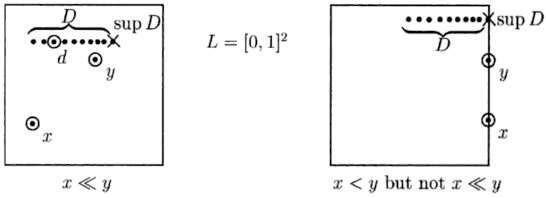
\includegraphics[scale=0.7]{figuurway.jpg}\\
  \caption{The ``Way Below''-relation on the lattice $[0,1]^2$.}\label{figuurway}
\end{figure}

\end{example}

\begin{theorem}
The direct product $\prod_{j \in J}L_j$ of a family dcpo's is again a dcpo with as way-below relation ($x, y \in \prod_{j \in J}L_j$):
$$x \ll y \Leftrightarrow x_j \ll y_j \;\forall j \in J \text{and } x_i = 0 \text{ for all but finitely many } i \in I$$
\end{theorem}

\begin{proof}
That being a dcpo is preserved under direct products is already proven in property \ref{directeproducten}. Now, we prove the characterization of the way-below relation in such a direct product.  Suppose first that $x \ll y$, for every finite set $F \subseteq J$, define $y^F \in \prod_{j \in J}L_j$ as follows:
\begin{equation*}
  y_j^F=\begin{cases}
    y_j & \text{if $j \in F $}\\
    0 & \text{if $j \not\in F $}
  \end{cases}
\end{equation*}
Than $\{y^F | F \subset J \text{ finite}\}$ is directed and its supremum is $y$. As $x \ll y$, there is some finite subset $F \subseteq J$ such that $x \leq y^F$, whence $x_j = 0 \;\forall j \not\in F$.
In order to show that $x_j \ll y_j \;\forall j \in J$, fix $j$ and consider any directed set $D \subset L_j$ such that $y_j \leq \sup D$. To every $d \in D$ we associate the element $\overline{d} \in \prod_{j \in J}L_j$ defined by:
\begin{equation*}
  \overline{d}_i=\begin{cases}
    d & \text{if $i = j$}\\
    y_i & \text{if $i \neq j $}
  \end{cases}
\end{equation*}
The family $\{\overline{d}|d\in D\}$ is directed and $y \leq \sup_{d \in D}\overline{d}$. As $x \ll y$, there is some $d \in D$ such that $x \leq \overline{d}$, whence $x_j \leq d$.\\

For the converse, suppose that $x_j \ll y_j \;\forall j \in J$ and that there is a finite set $F \subset J$ such that $x_j = 0 \;\forall j \not\in F$. Let $D$ be any directed set in $\prod_{j \in J}L_j$ such that $y \leq \sup D$. Then $y_j \leq \sup_{d\in D}d_j$ for every $j \in J$. As $x_j \ll y_j$, for every $j \in J$, there is a $d^j \in D$ such that $x_j \leq d^j_j$ (= $j$th component of $d^j$). As $D$ is directed, there is a $d \in D$ such that $d^j \leq d \;\forall j \in F$. Thus $x_j \leq d_j \;\forall j \in F$. As $x_j = 0 \;\forall j \not\in F$, we conclude that $x \leq d$. This proves that $x \ll y$.

\end{proof}


\begin{example}
If $L$ is a complete chain, and we consider the partially ordered \emph{direct power} $L^I$ of $L$ in the pointwise ordering, then in the complete lattice $L^I$ we find $x \ll y$ iff $x_i \ll y_i$ for all $i \in I$ and $x_i = 0$ for all but a finite number of indices $i$. This an immediate result from the previous theorem. When $I$ is infinite, this circumstance obviously justifies the ``way'' in ``way below".
\end{example}
\begin{example}
Consider a special case from the previous example, when $L$ is just the two element lattice and we can regard $L^I$ as the powerset lattice: in the powerset of $I$, the relation $A \ll B$ just means that $A$ is a finite subset of $B$.
\end{example}

\begin{example}
What does it mean if $x \ll x \; \forall x \in L$? Clearly, every \emph{finite poset} has this property. More generally it is necessary and sufficient that there be no strictly increasing infinite chains in the partial ordering, because the sup of such a chain cannot be compact. This is just the \emph{ascending chain condition} for $L$, and it is equivalent to saying that every nonempty subset contains a maximal element (and hence every directed set has a maximum).
\end{example}

\subsection{Domains}
\begin{definition}
A poset $L$ is called \emph{continuous} if $\downdownarrow x$ is directed with supremum $x$ for all $x \in L$.
\end{definition}

\begin{definition}
A dcpo which is continuous as a poset will be called a \emph{domain}.
\end{definition}


\begin{definition}
A subset $B$ of a dcpo $L$ is a \emph{basis} for $L$  if for all $x \in L, \{y \in B | y \ll x \}$ is directed with supremum $x$.
\end{definition}

\begin{lemma}
A dcpo $L$ is continuous iff it has a basis $B$.
\end{lemma}
\begin{proof}
If the dcpo $L$ is continuous take $B = L$. Conversely, if the dcpo $L$ has a basis $B$, take a random element $x \in L$, because $\{y \in B | y \ll x \}$ is directed with supremum $x$, $\downdownarrow x$ is also directed because every subset of $\downdownarrow x$  has at least the upper bound $x$. It's easy to see that $x$ is also the supremum of $\downdownarrow x$, because $\{y \in B | y \ll x \} = \downdownarrow x \cap B$ has as supremum $x$ and the set $ \downdownarrow x$ will only contain elements ``way below'' x.
\end{proof}

\begin{definition}
A poset is \emph{algebraic} if its compact elements form a basis. A poset is \emph{$\omega$-continuous} if it has a countable basis.
\end{definition}

\begin{example} \textbf{(The Interval Domain)}
The collection of compact intervals of the real line:
$$\mathcal{C}(\R) = \{[a, b] | a, b \in \R \text{ and } a \leq b \}$$
ordered under reverse inclusion
$$[a, b] \leq [c, d] \Leftrightarrow [c, d] \subseteq [a, b]$$
is a \emph{$\omega$-continuous} dcpo ($\omega$-domain). The supremum of a directed set $S \subset \mathcal{C}(\R)$ is $\cap S$.

If we take a look at the way below-relation then we can proof the relation is characterized by $$[a, b] \ll [c, d] \Leftrightarrow [c, d] \subset ]a, b[.$$ Let $I = \{]c-\epsilon, d + \epsilon[ | \epsilon > 0 \}$, than $I$ is directed with $\sup I = [c, d]$. If $[a, b] \ll [c, d]$, then there exists an $\epsilon > 0$, wherefore $]c-\epsilon, d + \epsilon[ \subset [a, b]$ which means $[c, d] \subset ]a, b[$. It follows that:
\begin{eqnarray*}
\downdownarrow [c, d] &= \{ [a, b] \subset \R | [a, b] \ll [c, d]  \} \\
&= \{ [a, b] \subset \R | [c, d] \subset ]a, b[  \}
\end{eqnarray*}
This set is obviously directed with supremum [c,d].
\end{example}

\begin{example} \textbf{(The Formal Ball Model}
Given a metric space ($X$, $d$), the formal ball model
$$\text{\textbf{B}}X = X \times [0, \infty[$$
is a poset when ordered via
$$(x, r) \leq (y, s) \Leftrightarrow d(x, y) \leq r - s.$$

The way below-relation can be characterized by $$(x, r) \ll (y, s) \Leftrightarrow d(x,y) < r - s.$$ Let $I$ be a subset of $X$, then $\text{\textbf{B}}I = I \times [0, \infty[$ is a subset of $\text{\textbf{B}}X$. This subset is directed,


\end{example}
\begin{theorem}
The direct product $\prod_{j\in J}L_j$ of a family domains $L_j, j \in J$ is itself a domain with as way-below relation ($x, y \in \prod_{j \in J}L_j$):
$$x \ll y \Leftrightarrow x_j \ll y_j \;\forall j \in J \text{and } x_i = 0 \text{ for all but finitely many } i \in I$$
\end{theorem}

\begin{proof}
In property \ref{directeproducten} we already proved that the direct product of a family dcpo\'s is itself a dcpo for the pointwise ordering, so the only thing that is left to prove is that if every dcpo in such a family is continuous, the direct product is also continuous. Take an element $(x_j)_{j\in J} \in \prod_{j \in J}L_j$, for every $j \in J$ it holds that $\downdownarrow x_j$ is directed with supremum $x_j$, this means that $\downdownarrow(x_j)_{j\in J}$ is also directed with supremum $(x_j)_{j\in J}$, which proves continuity.
\end{proof}


\begin{lemma}\label{lemmavoor}
If $x \ll z$ and if $z \leq \sup D$ for a directed set $D$ in a continuous poset $L$, then $x \ll d$ for some element $d \in D$.
\end{lemma}

\begin{proof}
Let $D$ be a directed set with $z \leq \sup D$, and let $I = \cup\{\downdownarrow d | d \in D\}$. By continuity, $\sup I = \sup D$ and, being a union of a directed family of ideals, $I$ is an ideal. Hence, if $x \ll z$, then $x \in I$ (immediate from the definitions), which means that $x \ll d$ for some $d \in D$.
\end{proof}

\begin{theorem}\label{interpolation}\textbf{(Interpolation property)} In a continuous posets L, the way-below relation satisfies the interpolation property $$x \ll z \Rightarrow \exists y: x \ll y \ll z.$$
\end{theorem}
\begin{proof}
This follows immediately from the previous lemma, by choosing $D = \downdownarrow z$ and recalling that $z = \sup \downdownarrow z$, by continuity of $L$.
\end{proof}

\section{Scott convergence}
In the introduction, we discussed the rich order theoretic structure of lattices, dcpo's and domains. We also introduced the way below-relation on this structures. The aim of this section is to introduce the Scott topology and its connection with convergence given in order theoretic terms by lower limits (or liminfs). Lower limits are defined on nets of dcpo's and will give meaning to the convergence of these nets. On the set of convergent nets we will be able to construct a topology that became famous as the Scott topology  (named after the mathematician Dana Scott). In general topology this type of definition is common in associating open sets with a class of nets given as convergent. It isn't surprising that this definition of the Scott topology on a dcpo will characterize rather than exhibit open sets. When defining the Scott topology on domains, the convergence of nets will be topological which will characterize domains in a nice way.

\subsection{$\mathcal{S}$-limits}
\begin{definition} \textbf{(Lower limit or liminf)} Let $L$ be a complete semilattice. For any net $(x_j)_{j\in J}$ we write
$$\liminf_j x_j = \sup_j \inf_{i \geq j x_i},$$
and call $\liminf_j x_j$ the \emph{lower limit} or \emph{liminf} of the net.
\end{definition}

\begin{definition} \textbf{($\mathcal{S}$-limit)} Let $\mathcal{S}$ denote the class of the pairs $((x_j)_{j\in J}, x)$ such that $x \leq \liminf_j x_j$ ($\mathcal{S} = \{((x_j)_{j\in J}, x) | x \leq \liminf_j x_j \}$ . For each such pair we say that $x$ is an $\mathcal{S}-limit$ of $(x_j)_{j \in J}$ and we write briefly $x \equiv_{\mathcal{S}} \lim x_j$.
\end{definition}
If we generalize this definition to dcpo's, we have to take into consideration that a dcpo can lack an infinium for each directed subset. This give rise to the notion of an \emph{eventual lower bound}.

\begin{definition}\textbf{(Eventual lower bound)} Let $L$ be a dcpo. An element $y \in L$ is an \emph{eventual lower bound} of a net $(x_j)_{j\in J}$ in $L$ if there exists $k \in J$ such that $y \leq x_j$ for all $j > k$.
\end{definition}

An equivalent definition for the class $\mathcal{S}$ is defined as:

\begin{definition}
 Let $\mathcal{S}$ denote the class of the pairs $((x_j)_{j\in J}, x)$ such that $x \leq \sup D$ for some directed set $D$ of eventual lower bounds of the net $(x_j)_{j\in J}$. For each such pair we say again that $x$ is an $\mathcal{S}-limit$ of $(x_j)_{j \in J}$.
\end{definition}

\begin{definition}If the set of all eventual lower bounds of $(x_j)_{j\in J}$ has a supremum which also a directed supremum of some subset off the set of eventual lower bounds (i.e. is an $\mathcal{S}$-limit of $(x_j)_{j\in J}$), then this supremum is called the \emph{lower limit} or the \emph{liminf} of the net, written $\liminf_j x_j$.
\end{definition}

The second definition of $\mathcal{S}$ and of the liminf for dcpo's, when applied to complete semilattices, agrees with the first definition of $\mathcal{S}$ and of the liminf for complete semilattices. Indeed if $\inf_{i \geq j}x_i$ exists for all $j \in J$, write $y_j = \inf_{i \geq j} x_i$. Then the collection $Y$ of all such $y_j$ is directed an the set of all eventual lower bounds is equal to $\downarrow Y$. Thus $\sup Y = \liminf_j x_j$.

\subsection{Convergence and topology}
We now use the general relation between \emph{convergence} and \emph{topology}. If on any set $L$ one is given an arbitrary class $\mathcal{L}$ of pairs $((x_j)_{j\in J}, x)$ consisting of a net and an element of $L$, then associated with $\mathcal{L}$ is a family of sets
$$\mathcal{O}(\mathcal{L}) = \{U \subseteq L | \text{ if } ((x_j)_{j\in J}, x) \in \mathcal{L} \text{ and } x \in U \text{ then eventually } x_j \in U\}.$$

\begin{property}
$\mathcal{O}(\mathcal{L})$ is a topology on $L$.
\end{property}
\begin{proof}
Clearly both $\emptyset$ and $L$ belong to $\mathcal{O}(\mathcal{L})$.

Take $A, B \in \mathcal{O}(\mathcal{L})$, let $((x_j)_{j\in J}, x) \in \mathcal{L}$ and $x \in A \cap B$, it follows that eventually $x_j \in A$ and eventually $x_j \in B$, in other words there exists elements $k_1, k_2 \in J$  such that for every $j \geq k_1$ it follows that $x_j \in A$ and for every $j \geq k_2$ it follows that $x_j \in B$. Define $k = k_1 \vee k_2$, than $\forall j \geq k: x_j \in A \cap B$. So $\mathcal{O}(\mathcal{L})$ is closed under the formation of finite intersections. A same argument can be used to proof that $\mathcal{O}(\mathcal{L})$ is also closed under the formation of arbitrary unions.
\end{proof}

By definition we know that, for any $((x_j)_{j\in J}, x) \in \mathcal{L}$, the element $x$ is a limit of the net $x_j$ relative to the topology $\mathcal{O}(\mathcal{L})$. Since however, $\emptyset$ and $L$ may very well be the only elements of $\mathcal{O}(\mathcal{L})$, what makes $\mathcal{O}(\mathcal{L})$ the indiscrete topology, we are obviously not saying very much; specific information information on $\mathcal{L}$ must become available before one can hope to get a close link between $\mathcal{L}$ and $\mathcal{O}(\mathcal{L})$. Fortunately, in our present situation, we do have specific information about our class $\mathcal{S}$. We begin exploiting by characterizing the sets $U \in \mathcal{O}(\mathcal{S})$.

\begin{theorem}\label{scottprot} Let $L$ be dcpo and $U \subset L$. Then $U \in \mathcal{O}(\mathcal{S})$ iff the following two conditions are satisfied:
\begin{enumerate}[(i)]
    \item $U = \uparrow U$;
    \item $\sup D \in U$ implies $D \cap U \neq \emptyset$ for all directed set $D \subseteq L$.
\end{enumerate}
\end{theorem}
\begin{proof}
First, suppose $U \in \mathcal{O}(\mathcal{S})$. To prove (i), assume $u \in U$ and $u \leq x$. then $u \leq x = \liminf  x$ with the constant net $(x)$ with value $x$, so by definition $((x), u) \in \mathcal{S}$. Since we have that $u \in U \in \mathcal{O}(\mathcal{S})$, we conclude from the definition of $\mathcal{O}(\mathcal{S})$ that the net $(x)$ must be eventually in $U$. This means $x \in U$. So $U = \uparrow U$.

In order to prove (ii), let $D$ be a directed set in $L$ with $\sup D \in U$. Consider the net $(x_d)_{d \in D}$ with $x_d = d$. Now $inf_{c\geq d} x_c = d$, and thus $\liminf_{d \in D} x_d = \sup D \in U \in \mathcal{O}(\mathcal{S})$. Since $((x_d)_{d \in D}, \sup D) \in \mathcal{S}$, we conclude that $d = x_d$ is eventually in $U$; whence $D \cap U \neq \emptyset$.\\

Second, suppose that $U$ satisfies (i) and (ii). We take $((x_j)_{j \in J}, x) \in \mathcal{S}$ with $x \in U$, and we must show that $x_j$ is eventually in $U$. By the definition of $\mathcal{S}$, we have $x \leq \sup D$ for some directed set $D$ of eventual lower bounds of $(x_j)_{j \in J}$. Then $x \in U$ implies $\sup D \in U$ by (i), and then $d \in U$ for some $d \in D$ by (ii). By definition $d \leq x_i$, for all $i \geq j$ for some $j \in J$. Again by (i), $x_i \in U$ for all $i \geq j$. Thus $U \in \mathcal{O}(\mathcal{S})$.
\end{proof}

\begin{definition}\textbf{(Scott topology)} A subset $U$ of a dcpo $L$ is called \emph{Scott open} iff it satisfies the conditions of the previous theorem. the complement of a Scott open set is called \emph{Scott closed}. The collection of all Scott open subset of $L$ will be called the \emph{Scott topology} of L and will be called the \emph{Scott topology} of $L$ and will be denoted by $\sigma(L)$.
\end{definition}

\begin{definition}\textbf{($\mathcal{S}$-property)}
We say that a subset $X$ of a dcpo $L$ has the $\mathcal{S}$-property provided that the following condition is satisfied:
$$\text{If } \sup D \in X \text{ fro any directed set } D \text{, then there is a} y \in D \text{ such that } x \in X \forall x \in D \text{ with } x \geq y.$$
\end{definition}

\begin{theorem}If any dcpo L we have the following properties:
\begin{enumerate}[(i)]
    \item a set is Scott closed iff it is a lower set closed under directed sups,
    \item $\downarrow x = \{\overline{x}\}$ (closure with respect to $\sigma{L}$) for all $x \in L$,
    \item $\sigma(L)$ is a $T_0$ space,
    \item every upper set is the intersection of its Scott open neighborhoods,
    \item a set is Scott open iff it is an upper set satisfying the $\mathcal{S}$-property,
    \item every lower set has the $\mathcal{S}$-property,
    \item the collection of all subsets having the $\mathcal{S}$-property is a topology.
\end{enumerate}
\end{theorem}

\begin{proof}
\begin{enumerate}[(i)]
    \item $A \subseteq L$ is a lower set iff $L \setminus A$ is an upper set, and $L \setminus A$ satisfies the second condition in Theorem \ref{scottprot} iff $A$ closed under directed sups.
    \item We have that $\downarrow x$ is the smallest lower set containing $x$, and it happens to be closed under directed sups. It follows from (i) that $\downarrow x$ is the smallest Scott closed set that contains $x$.
    \item If $\{\overline{x}\} = \{\overline{y}\}$, then $\downarrow x = \downarrow y$ by (ii); thus $x = y$, which proves that $\sigma(L)$ is a $T_0$-space.
    \item Every upper set $B$ is the intersection of the sets $L \setminus \downarrow x$ where $x \in L \setminus B$ ($B = \cap_{x \in L \setminus B} L \setminus \downarrow x$). When applying (ii), these sets are Scott open.
    \item This follows immediately from the second condition in Theorem \ref{scottprot}.
    \item Let $X$ be a lower set, $D$ a directed subset of $L$ with $\sup D \in X$ then it holds for all $d \in D$ that $d \leq \sup D$ which means that $d \in X = \downarrow X$.
    \item First, $\emptyset$ and $L$ satisfy the $\mathcal{S}$-property. Let us now proof that the $\mathcal{S}$-property stays satisfied under the formation of finite intersections with the $\mathcal{S}$-property. Take the sets $A, B \subseteq L$ which satisfy the $\mathcal{S}$-property, and take $D \subseteq L$ a directed subset of $L$ with $\sup D \in A \cap B$. Of course $\sup D \in A$ and $\sup D \in B$, so there exists elements $y_1, y_2 \in D$ such that $\forall x \geq y_1$ it follows that $x \in A$ and $\forall x \geq y_2$ it follows that $x \in B$. Let $y = y_1 \vee y_2$, then it holds for all $x \in D \geq y$ that $x \in A \cap B$. The fact that the $\mathcal{S}$-property is also satisfied under the formation of arbitrary unions of sets with the $\mathcal{S}$-property is provable in the same way.
\end{enumerate}
\end{proof}
\begin{example}
If $L$ is the unit interval: $L = [0,1]$, then $L$ is a complete chain, hence a dcpo.  Any Scott open set has the form $]x,1]$ if $0 \leq x \leq 1$ or $[0, 1]$. $]x, 1]$ is Scott open by the second condition of the previous theorem because $]x, 1] = \uparrow x \setminus \{x\} = L \setminus \downarrow x$. $[0,1]$ is Scott open because it's an upper set that satisfies trivially the $\mathcal{S}$-property.

Conversely, let $U$ be a Scott open set then it follows from the first condition from Theorem \ref{scottprot} that $U = \uparrow U$, this means that $U$ can be $]x, 1]$ or $[x, 1]$. But consider $D = L \setminus [x, 1]$ with $x \neq 0$, $D$ is clearly a directed set with $\sup D = x \in U$ but $U \cap D = \emptyset$ so $[x, 1]$ with $x \neq 0$ doesn't satisfy the conditions to be Scott open. The only Scott open sets are thus $]x, 1]$ with $0 \leq x \leq 1$ together with $L$.
\end{example}

\begin{example}
Let $L = [0, 1]^2$, the square with the pointwise ordering, which is of course a dcpo because it's already a continuous lattice. From the previous example, we know that $\sigma([0,1]) = \{]x, 1] | 0 \leq x \leq 1 \} \cup \{[0,1]\}$. An interesting question is now: is the product topology on L generated by the rectangles $]x_1, 1] \times ]x_2, 1]$ (with $x_1, x_2 \in [0, 1])$ also a Scott topology on $L$? Indeed, for an open set $U$ of the product topology it holds clearly that $U = \uparrow U$. For each directed set $D = D_1 \times D_2 \subseteq L$ with $\sup D = (\sup D_1, \sup D_2) \in U$ it holds that there exists Scott open sets $]x_1, 1]$ and $]x_2, 1]$ of $[0, 1]$ with $]x_1, 1] \times ]x_2, 1] \subset U$ such that $\sup D_1 \in ]x_1, 1]$ and $\sup D_2 \in ]x_2, 1]$. It follows that $D_1 \cap ]x_1, 1] \neq \emptyset$ and $D_2 \cap ]x_2, 1] \neq \emptyset$ and thus $D \cap ]x_1, 1] \times ]x_2, 1] \subseteq U \neq \emptyset$.
\end{example}

\begin{example}
We can also put another topology on $L = [0,1]^2$, in this topology a subset $U$ is Scott open iff it is an upper set and its open in the ordinary topology induced by the plane. Figure \ref{scottplane} shows a picture of these open sets. That this topology is indeed a Scott topology is easy to see: let $U$ be a Scott open set but not open for the ordinary topology induced by the plane, then there exist an element $u \in U$ for which each ball centered at $u$ is not contained in $U$. Consider now the directed set $D \subseteq L\setminus U$, with $\sup D = u$. It follows that $U$ is also not Scott open. Conversely, if $U = \uparrow U$ is not Scott open, then there exists a directed set $D \subseteq L$ with $\sup D \in U$ but with $D \cap U = \emptyset$, which means that for all balls centered at $\sup D$ it holds that they aren't a subset of $U$, which means that $U$ is not open for the ordinary topology on $[0,1]^2$. So we see that in this topology every Scott open set of $[0,1]^2$ is the union of open upper rectangles. Note that these rectangles are the intersection of two sets of the form $L\setminus \downarrow x$.
\end{example}
\begin{example}
On the chain $L = \{0, 1\}$, the Scott topology equals the Sierpinski topology, $\sigma(L) = \{\emptyset, \{1\}, L\}$.
\end{example}

\begin{theorem}\label{begindomein}
If $L$ is a domain, then all sets $\upuparrow x$ for $x \in L$ are Scott open. Conversely, if $L$ is a dcpo and $y \in \int(\uparrow x)$, then $x \ll y$.
\end{theorem}

\begin{proof}
Let $D$ be a directed set with $\sup D \in \upuparrow x$, then Lemma \ref{lemmavoor} implies the existence of a $d \in D$ such that $x \ll d$ en thus $d \in \upuparrow x$. Hence $\upuparrow x$ is Scott open by definition.

Suppose $L$ is a dcpo and $y \in \int(\uparrow x)$, if $D$ is a directed set with $y \leq \sup D$, then $\sup D \in \int(\uparrow x)$ because $\int(\uparrow x)$ is Scott open and $x \leq d \leq \sup D$. It follows that $D \cap \int(\uparrow x) \neq \emptyset$. Hence, there exists a $d \in D$ with $d \in \int(\uparrow x)$, thus $x \leq d$ and it follows that $x \ll y$.
\end{proof}
\begin{remark}
The notation $\int(S)$ is used to indicate the interior of a set $S$ and is defined as the set of all interior points of $S$, or, in other words, the largest  open set contained in $S$. From the previous theorem we can thus conclude that, when $L$ is a domain, for each $x \in L$ it holds that $\int(\uparrow x) = \upuparrow x$.
\end{remark}
In order to conclude this section, we must return to the discussion of the concept of convergence and investigate whether the Scott topology (which we derived from a convergence concept) is in fact adequate to describe in topological terms the $\mathcal{S}$-convergence. If $\mathcal{S}$ is precisely the class of convergent nets for the Scott topology, then we say that $\mathcal{S}$ is topological.

\begin{theorem}
Let $L$ be a domain. Then $x \equiv_{\mathcal{S}} \lim x_j$ iff the net $(x_j)_{j\in J} \rightarrow x$ with respect to the Scott topology $\sigma(L)$. In particular, the $\mathcal{S}$-convergence is topological.
\end{theorem}
\begin{proof}
By definition of the Scott topology, if $x \equiv_{\mathcal{S}} \lim x_j$, then $(x_j)_{j\in J} \rightarrow x$ with respect to $\sigma(L)$.
 
Conversely, suppose that we have a convergent net $(x_j)_{j\in J} \rightarrow x$ in the Scott topology. For each $y \in \downdownarrow x$, we have that $\upuparrow y$ is a Scott open set containing $x$ by Theorem \ref{begindomein}. Thus the net $(x_j)_{j\in J}$ is eventually in $\upuparrow y$, and hence $y$ is an eventual lower bound for the net. Since $\downdownarrow x$ is directed and has supremum $x$, we have $((x_j)_{j\in J}, x) \in \mathcal{S}$.
\end{proof}
If the $\mathcal{S}$-convergence is topological in a dcpo, the dcpo is a domain, thus the converse is also true:
\begin{lemma}
Let L be a dcpo, if the $\mathcal{S}$-convergence is topological, then $L$ is a domain.
\end{lemma}

\begin{proof}
By Lemma \ref{scottprot} the topology arising from $\mathcal{S}$-convergence, is the Scott topology. Thus if $\mathcal{S}$-convergence is topological, we must have $x \equiv_{\mathcal{S}} \lim x_j$ iff the net $(x_j)_{j\in J} \rightarrow x$ with respect to $\sigma(L)$. Let $x \in L$. Define $$I = \{(U,n,a) \in \mathcal{N}(x) \times \N \times L | a \in U\},$$
where $\mathcal{N}(x)$ consists of all Scott open sets containing $x$, and define an order on $I$ to be the lexicographic order on the first two coordinates, that is, $(U, m, a) < (V, n, b)$ iff $V$ is a proper subset of $U$ or $U = V$ and $m < n$. Let $x_i = a$ for $i = (U, n, a) \in I$ define the net. Then it is easy to see that $(x_i)_{i \in I}$ converges to $x$ in the Scott topology. Thus $x \equiv_\mathcal{S} \lim x_i$, and we conclude that there exists a directed set $D$ of eventual lower bounds of $(x_i)_{i\in I}$ such that $x \leq \sup D$. Let $d \in D$. Then there exists $i = (U, m, a) \in I$ such that $(V, n, b) = j \geq i$ implies $d \leq b$. In particular, we have $(U, m + 1, b) > (U, m, a)$ for all $b \in U$, and thus $d$ is a lower bound for $U$, i.e., $x \in \int(\uparrow d)$. By Theorem \ref{begindomein}, $d \ll x$. Since $D$ is directed with supremum greater than or equal to $x$, we conclude that $x$ is the directed supremum of $D \subseteq \downdownarrow x$. Since $x$ was arbitrary, we conclude that $L$ is a domain.
\end{proof}

\subsection{The Scott topology of domains}
So now we know that for a dcpo $L$, that $L$ being a domain is equivalent with saying that the $\mathcal{S}$-convergence is topological for the Scott topology $\sigma(L)$. This means that domains are extremely useful to study lower semicontinuity completely in topological terms.

\begin{theorem}
Let $L$ be a domain
    \begin{enumerate}[(i)]
        \item An upper set $U$ is Scott open iff for every $x \in U$ there is a $u \in U$ such that $u \ll x$.
        \item The sets of the form $\upuparrow x$, $u \in L$, form a basis for the Scott topology. In particular, each point $x \in L$ has a $\sigma(L)$ neighborhood basis consisting of the sets $\upuparrow x$ with $u \ll x$.
        \item With respect to $\sigma(L)$, we have $\int(\uparrow x) = \upuparrow x$.
        \item With respect to $\sigma(L)$, we have for any subset $X \subseteq L$
        $$\int(X) = \displaystyle\bigcup{\{\upuparrow u \; | \upuparrow u \subseteq X\}}$$.
    \end{enumerate}
\end{theorem}
\begin{proof}
\begin{enumerate}[(i)]
        \item Let $U$ be Scott open and $x \in U$. As in a domain the set $\downdownarrow x$ is directed and has supremum $x$, we conclude that there is a $u \ll x$ with $u \in U$ by the second condition of Lemma \ref{scottprot}.
            
            If conversely for every $x \in U$ there is a $u \in U$ such that $u \ll x$ then $U$ is the union of the sets $\upuparrow u$, $u \in U$, which are Scott open by Theorem \ref{begindomein}; hence, $U$ is Scott open.
        \item Follows immediately of (i).
        \item If $y \in \int(\uparrow x)$, then by (i) there is a $u \in \uparrow x$ with $u \ll y$. But then $y \in \upuparrow x$. Obviously $\upuparrow x \subseteq \int(\uparrow x)$.
        \item Follows immediately of (ii).
    \end{enumerate}
\end{proof}

\subsection{Scott-Continuous Functions}


\newpage
\begin{thebibliography}{99}
\bibitem{1} G. Gierz, K. H. Hofmann, K. Keimel, J. D. Lawson, M. W. Mislove, D. S. Scott, {\em Continuous Lattices and Domains}, Cambridge University Press, Cambridge (2003).
\bibitem{2} E. Colebunders, \emph{Topologie}, Vrije Universiteit Brussel, 2012.
\bibitem{3} K. Martin, \emph{A Foundation for Computation}, July 2000
    \end{thebibliography}
\end{document}

